\section{Backpropagation in the Simply Typed Lambda-Calculus with Linear Negation}
Backpropagation is a classic automatic differentiation algorithm computing the gradient of functions specified by a certain class of simple, first-order programs, called \emph{computational graphs}. 
Recent years have witnessed the quick growth of a research field called \emph{differentiable programming}, the aim of which is to express computational graphs more synthetically and modularly by resorting to actual programming languages endowed with control flow operators and higher-order combinators, such as map and fold. In this paper, we extend the backpropagation algorithm to a paradigmatic example of such a programming language: we define a compositional program transformation from the simply-typed lambda-calculus to itself augmented with a notion of linear negation, and prove that this computes the gradient of the source program with the same efficiency as first-order backpropagation.

\subsection{Introduction}
In the past decade there has been a surge of interest in so-called deep learning, a class of machine learning methods based on multi-layer neural networks. The term “deep” has no formal meaning, it is essentially a synonym of “multi-layer”, which refers to the fact that the networks have, together with their input and output layers, at least one internal (or “hidden”) layer of artificial neurons. Technically, the neurons are just functions $\mathbb{R}^n \rightarrow \mathbb{R}$ of the form $(x_1,..., x_m) \rightarrow \sigma(\sum^{m}_{i=1} w_i \cdot x_i)$, where $\sigma: \mathbb{R}\rightarrow\mathbb{R}$ is some \emph{activation function} and $w_1,..., w_m \in \mathbb{R}$ are the \emph{weights} of the neuron.

Feed-forward, multi-layer neural networks are known to be universal approximators: any continuous function $f: K \rightarrow \mathbb{R}$ with $K \subset \mathbb{R}^k$ compact may be approximated to an arbitrary degree of precision by a feed-forward neural network with one hidden layer, as long as the weights are set properly. This leads us to the following two questions related to each other:
\begin{enumerate}
	\item How to efficiently train a neural network? i.e., how to find the right weights as quickly as possible?
	\item How to select and, if necessary, modify or design network architectures adapted to a given task?
	Since the quality of an architecture is also judged in terms of training efficiency, this problem is actually interlaced
	with the previous one.
\end{enumerate}

\subsubsection{How to efficiently train a neural network?} The first question is generally answered in terms of the gradient descent algorithm (or some variant thereof). 

\paragraph{Gradient Descent Algorithm} The Gradient Descent Algorithm finds local minima of a function $G : \mathbb{R}^n \rightarrow \mathbb{R}$ using its gradient $\nabla G$. The algorithm starts by choosing a point $\mathbf{w}_0 \in \mathbb{R}^n$. Under certain assumptions, if $\nabla G(\mathbf{w}_0)$ is close to zero then $\mathbf{w}_0$ is within a sufficiently small neighborhood of a local minimum. Otherwise, we know that $G$ decreases most sharply in the opposite direction of $\nabla G(\mathbf{w}_0)$, and so the algorithm sets $\mathbf{w}_1 := \mathbf{w}_0 - \rho \nabla G(\mathbf{w}_0)$ for a suitable step rate $\rho >0$, and repeats the procedure from $\mathbf{w}_1$ .

\paragraph{AD and efficient training of neural networks} So, regardless of the architecture, efficiently training a neural network involves efficiently computing gradients. The interest of gradient descent, however, goes well beyond deep learning, into fields such as physical modeling and engineering design optimization, each with numerous applications. It is thus no wonder that a whole research fie
known as automatic differentiation (AD for short), developed around the computation of gradients. In AD, the setting of neural networks is generalized to computational graphs, which are arbitrarily complex compositions of nodes computing basic functions and in which the output of a node may be shared as the input of an unbounded number of nodes.

The key idea of AD is to compute the gradient of a computational graph by accumulating in a suitable way the
partial derivatives of the basic functions composing the graph. This rests on the mathematical principle known as
\emph{chain rule}, giving the derivative of a composition $f \circ g$ from the derivatives of its components $f$ and $g$. Formally, the chain rule states that

$$\forall r \in \mathbb{R} \quad \quad (g \circ f)' (r) = g'(f(r)) \cdot f'(r)$$

There are two main “modes” of applying this rule in AD, either forward, propagating derivatives from inputs to outputs, or backwards, propagating derivatives from outputs to inputs. If $G$ is a computational graph with $n$ inputs and $m$ outputs invoking $|G|$ operations, forward mode computes the Jacobian of $G$ in $O(n |G|)$ operations, while reverse mode requires $O(m |G|)$ operations. In deep learning, as the number of layers increases, $n$ becomes astronomical (millions, or even billions) while $m = 1$, hence the reverse mode is the method of choice and specializes in what is called the backpropagation algorithm. Today, AD techniques are routinely used in the industry through deep learning frameworks such as TensorFlow and PyTorch.


\subsubsection{How to select and modify or design network architectures adapted to a given task?}
The interest of the programming languages (PL) community in AD stems from the second deep learning question mentioned above, namely the design and manipulation of (complex) neural network architectures. As it turns out, these are being expressed more and more commonly in terms of actual programs. Although these programs always reduce, in the end, to computational graphs, these latter are inherently static and therefore inadequate to properly describe something which is in reality, a dynamically-genereted neural network.

In PL-theoretic terms, this amounts to fixing a reduction strategy, which cannot always be optimal in terms of efficiency. There is also a question of modularity: if gradients may only be computed by running programs, then we are implicitly rejecting the possibility of computing gradients modularly, because a minor change in the code might result in having to recompute everything from scratch, which is clearly unsatisfactory.

\subsubsection{Goal}
Define a compositional program trasformation $\stackrel{\leftarrow}{D}$ extending the backpropagation algorithm from computational graph to general simply typed $\lambda$-terms. Our framework is purely logical and therefor offer the possibility of importing tool from semantics, type systems and rewriting theory.

\subsection{A Crash Course in Automatic Differentiation}

\subsubsection{What is Automatic Differentiation?}
Automatic differentiation (or AD) is the science of efficientlly computing the derivative of (a restricted class of) programs. Such programs may be represented as directed acyclic hypergraphs, called \emph{computational graphs}, whose nodes are variables of type $\mathbb{R}$ and whose hyperedges are labelled by functions drawn from some finite set of interest with the restriction that hyperedges have exactly one targetnode and that each node is the target of at most one hyperedge. The basic idea is that nodes that are not target of any hyperedge represent input variables, nodes which are not source of any hyperedge represent outputs, and a hyperedge $x_1, \dots, x_k \xrightarrow{f} y$ represents an assignment $y:= f(x_1,\dots, x_k)$. So that a computational graph with $n$ inputs and $m$ outputs represents a function of type $\mathbb{R}^n\rightarrow \mathbb{R}^m$. 

In terms of programming languages, we may define computational graphs as generated by
$$ F, G ::= x \mbox{ }|\mbox{ }  f(x_1,...,x_k) \mbox{ }|\mbox{ }  \mathtt{let} \mbox{ } x = G \mbox{ } \mathtt{in} \mbox{ }F \mbox{ }|\mbox{ }  (F,G) $$

where $x$ range over ground variables and $f$ over a set of real function symbols. The $\mathtt{let}$ binders are necessary to represents \emph{sharing}. The set of real function symbols consists of one nullary symbol for every real number plus finitely many non-nullary symbols for actual functions, we may write $f(G_1,\dots.G_n)$ as a syntactic sugar for $\mathtt{let} \mbox{ } x_1 = G_1 \mbox{ } \mathtt{in} \mbox{ } \dots \mbox{ } \mathtt{let} \mbox{ } x_n = G_n \mbox{ } \mathtt{in}  \mbox{ } f(x_1,...,x_n)$. 

\paragraph{Example} For example, the computational graph that represents the function $(x_1, x_2) \mapsto sin((x_1-x_2)^2)$ and its corresponding term are described in Figure~\ref{compGraph2}.

\begin{figure}[h!]
	\centering
	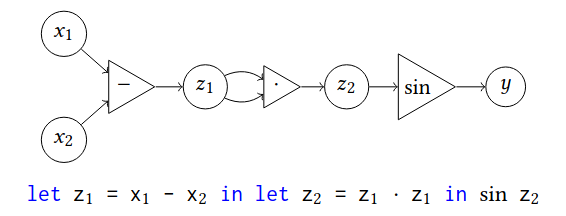
\includegraphics[scale=0.5]{img/compGraph2}
	\caption{Computational graph of the function $f(x_1,x_2)=sin((x_1-x_2)^2)$ and its corresponding term. Nodes are drawn as circles, 			hyperedges as triangles.}
	\label{compGraph2}
\end{figure}

\subsubsection{Forward Mode AD}

\subsubsection{Symbolic AD}

\subsubsection{Reverse Mode AD or Backpropagation}

\subsubsection{Symbolic Backpropagation and the Compositionality Issue}